\newpage
\appendix

% \iffalse
% Temporarily hidden while the main draft focuses on the NKL-only diagnostic.
% The CCR/log-elasticity algebra may be restored later if the main text
% reintroduces CCR as a central diagnostic.

\section{Environments, Tool Configurations, And Task Examples}
\label{app:envs}

In this work, we use the following three environments and task types:
ALFWorld~\citep{shridhar2021alfworld}, Multi-Hop Search (consisting of several sub-benchmarks including PopQA~\citep{mallen2023popqa}, NQ~\citep{kwiatkowski2019natural}, 2WikiMultiHopQA~\citep{ho2020twowiki}, HotpotQA~\citep{yang2018hotpotqa}), and WebShop~\citep{yao2022webshop}.

For the student and teacher models, we explicitly activate the ``thinking'' mode, so each model turn consists of a segment of chain-of-thought and a tool call.
Client-side validation rejects malformed or inadmissible actions before they reach the
environment so a bad action does not consume a real step.
All experiments are conducted on 32 NVIDIA H20 GPUs, each with 80 GB of memory.

\subsection{Environment Details}

\subsubsection{ALFWorld (Embodied Household Planning)}
\label{app:envs:alfworld}

\textbf{Tool / action space.} A single tool \texttt{alfworld\_step(action: str)}; the
action is a natural-language household command from the templates: \texttt{go to
\{loc\}}, \texttt{take \{obj\} from \{loc\}}, \texttt{put \{obj\} in/on \{loc\}},
\texttt{open/close \{loc\}}, \texttt{use \{loc\}}, \texttt{clean/heat/cool \{obj\} with
\{loc\}}, \texttt{examine \{x\}}, \texttt{inventory}, \texttt{look}. The tool returns
the new TextWorld observation plus a refreshed list of admissible commands; actions not
in the admissible set are rejected client-side.

\textbf{Environment.} A FastAPI server wraps TextWorld~\citep{cote2018textworld} with a
spawned worker pool. The six task types are \texttt{pick\_and\_place},
\texttt{pick\_clean\_then\_place}, \texttt{pick\_heat\_then\_place},
\texttt{pick\_cool\_then\_place}, \texttt{look\_at\_obj\_in\_light}, and
\texttt{pick\_two\_obj\_and\_place}; evaluation uses the \texttt{valid\_unseen}
(out-of-distribution) split. The reward is \textbf{binary} ($1$ on goal completion,
else $0$).

\textbf{Task example.}
\begin{verbatim}
[system] You are an AI agent operating in a household environment. You can
interact with objects and navigate between locations using the alfworld_step tool.
[user]   Your task is to: put a clean mug in coffeemachine.
[assistant -> alfworld_step] {"action": "go to countertop 1"}
[tool]   On the countertop 1 you see a mug 1, a knife 1, ...
[assistant -> alfworld_step] {"action": "take mug 1 from countertop 1"}
[tool]   You pick up the mug 1 from the countertop 1.
[assistant -> alfworld_step] {"action": "clean mug 1 with sinkbasin 1"} ...
\end{verbatim}

\subsubsection{Multi-Hop Search}
\label{app:envs:searchr1}

\textbf{Tool / action space.} We instantiate Multi-Hop Search with a Search-R1-style interface \citep{jin2025searchr1}. A single retrieval tool
\texttt{search\_r1/search(query: str)} POSTs the query to a dense-retrieval server and returns the top-$k$ passages
formatted as \texttt{Doc i(Title: ...) ...}. The model
reasons in \texttt{<think>...</think>}, issues retrieval via the search tool (or the
equivalent \texttt{<search>...</search>} text channel), receives results in
\texttt{<information>...</information>}, and emits the final answer in
\texttt{<answer>...</answer>}.

\textbf{Environment.} The retrieval endpoint serves
a fixed Wikipedia corpus; rollouts are capped at \texttt{max\_turns}=50, allowing many
search--read hops. The reward is \textbf{exact match (EM)} of the extracted
\texttt{<answer>} against the gold answer.

\textbf{Sub-benchmarks.} The held-out Multi-Hop Search test set is a mixture of
four QA sources: \texttt{PopQA}~\citep{mallen2023popqa},
\texttt{Natural Questions} (NQ)~\citep{kwiatkowski2019natural},
\texttt{2WikiMultiHopQA}~\citep{ho2020twowiki}, and
\texttt{HotpotQA}~\citep{yang2018hotpotqa}. PopQA and NQ provide open-domain
retrieval questions, while 2WikiMultiHopQA and HotpotQA require chained
retrievals where a later query depends on an earlier passage, making the
evaluation mixture cover both direct retrieval and long-horizon dependency
cases.

\textbf{Task example.}
\begin{verbatim}
[user] Answer the question. Reason in <think>...</think>; if you lack knowledge,
search via <search> query </search> and read the returned <information>...
</information>; give the final answer in <answer>...</answer>.
Question: Who is the director of the film that won Best Picture in the year
Titanic was released?
[assistant] <think>I need the Best-Picture winner of 1997.</think>
            <search> 1997 Academy Award Best Picture winner </search>
[tool]      <information>Doc 1(Title: Titanic (1997 film)) ... won Best Picture ...
            </information>
[assistant] <think>Director of Titanic is James Cameron.</think>
            <answer> James Cameron </answer>
\end{verbatim}

\subsubsection{WebShop (Web Navigation / Online Shopping)}
\label{app:envs:webshop}

\textbf{Tool / action space.} The agent operates a single tool \texttt{webshop\_step(action: str)} with two formats: \texttt{search[<keywords>]} for query input (when a search bar is available), and \texttt{click[<button>]} to interact with one of the currently visible buttons (e.g., product ID, attribute options like ``x-large'', or navigation buttons such as \texttt{Buy Now}, \texttt{Next >}, etc.). The tool outputs the updated page view and available actions. Invalid clicks are blocked on the client side.

\textbf{Environment.} A FastAPI server wraps AgentGym's
\texttt{agentenv\_webshop}~\citep{xi2025agentgym}. An episode proceeds search $\to$ inspect results $\to$ open a
product $\to$ select attributes $\to$ \texttt{click[Buy Now]}. The reward is a
\textbf{dense terminal score in $[0,1]$} reflecting partial credit for matching the
requested product type, attributes, options, and price; only the terminating
\texttt{Buy Now} carries reward, and a machine-parseable
\texttt{[WEBSHOP\_FINAL\_SCORE=...]} marker is appended for the reward path.

\textbf{Task example.}
\begin{verbatim}
[user] Instruction: I am looking for a milk chocolate of 1 pound size in a single
pack for valentine day, and price lower than 40 dollars.
Available actions: search[<your keywords>]
[assistant -> webshop_step] {"action": "search[valentine milk chocolate 1 pound
single pack]"}
[tool]  [Results] B07... Valentine Milk Chocolate 1 lb ... $19.99  (clickables:
        "B07...", "Next >", "Back to Search")
[assistant -> webshop_step] {"action": "click[B07...]"}
[tool]  ... (clickables: "1 pound", "Buy Now", "Description", ...)
[assistant -> webshop_step] {"action": "click[Buy Now]"}
[tool]  Episode finished with score=1.000.  [WEBSHOP_FINAL_SCORE=1.000000]
\end{verbatim}

\subsection{Task-Specialized Teacher Training}
\label{app:teacher-grpo}

We train task-specialized teachers using GRPO~\citep{shao2024deepseekmath} on the three environments.
Figure~\ref{fig:teacher-grpo-val} reports the validation dynamics of the
task-specialized teachers used in the main experiments. All curves report avg@4 accuracy. ALFWorld and WebShop use Qwen3-8B-GRPO
teachers, while Multi-Hop Search uses a Qwen3.5-9B-GRPO teacher.

\begin{figure*}[htbp]
  \centering
  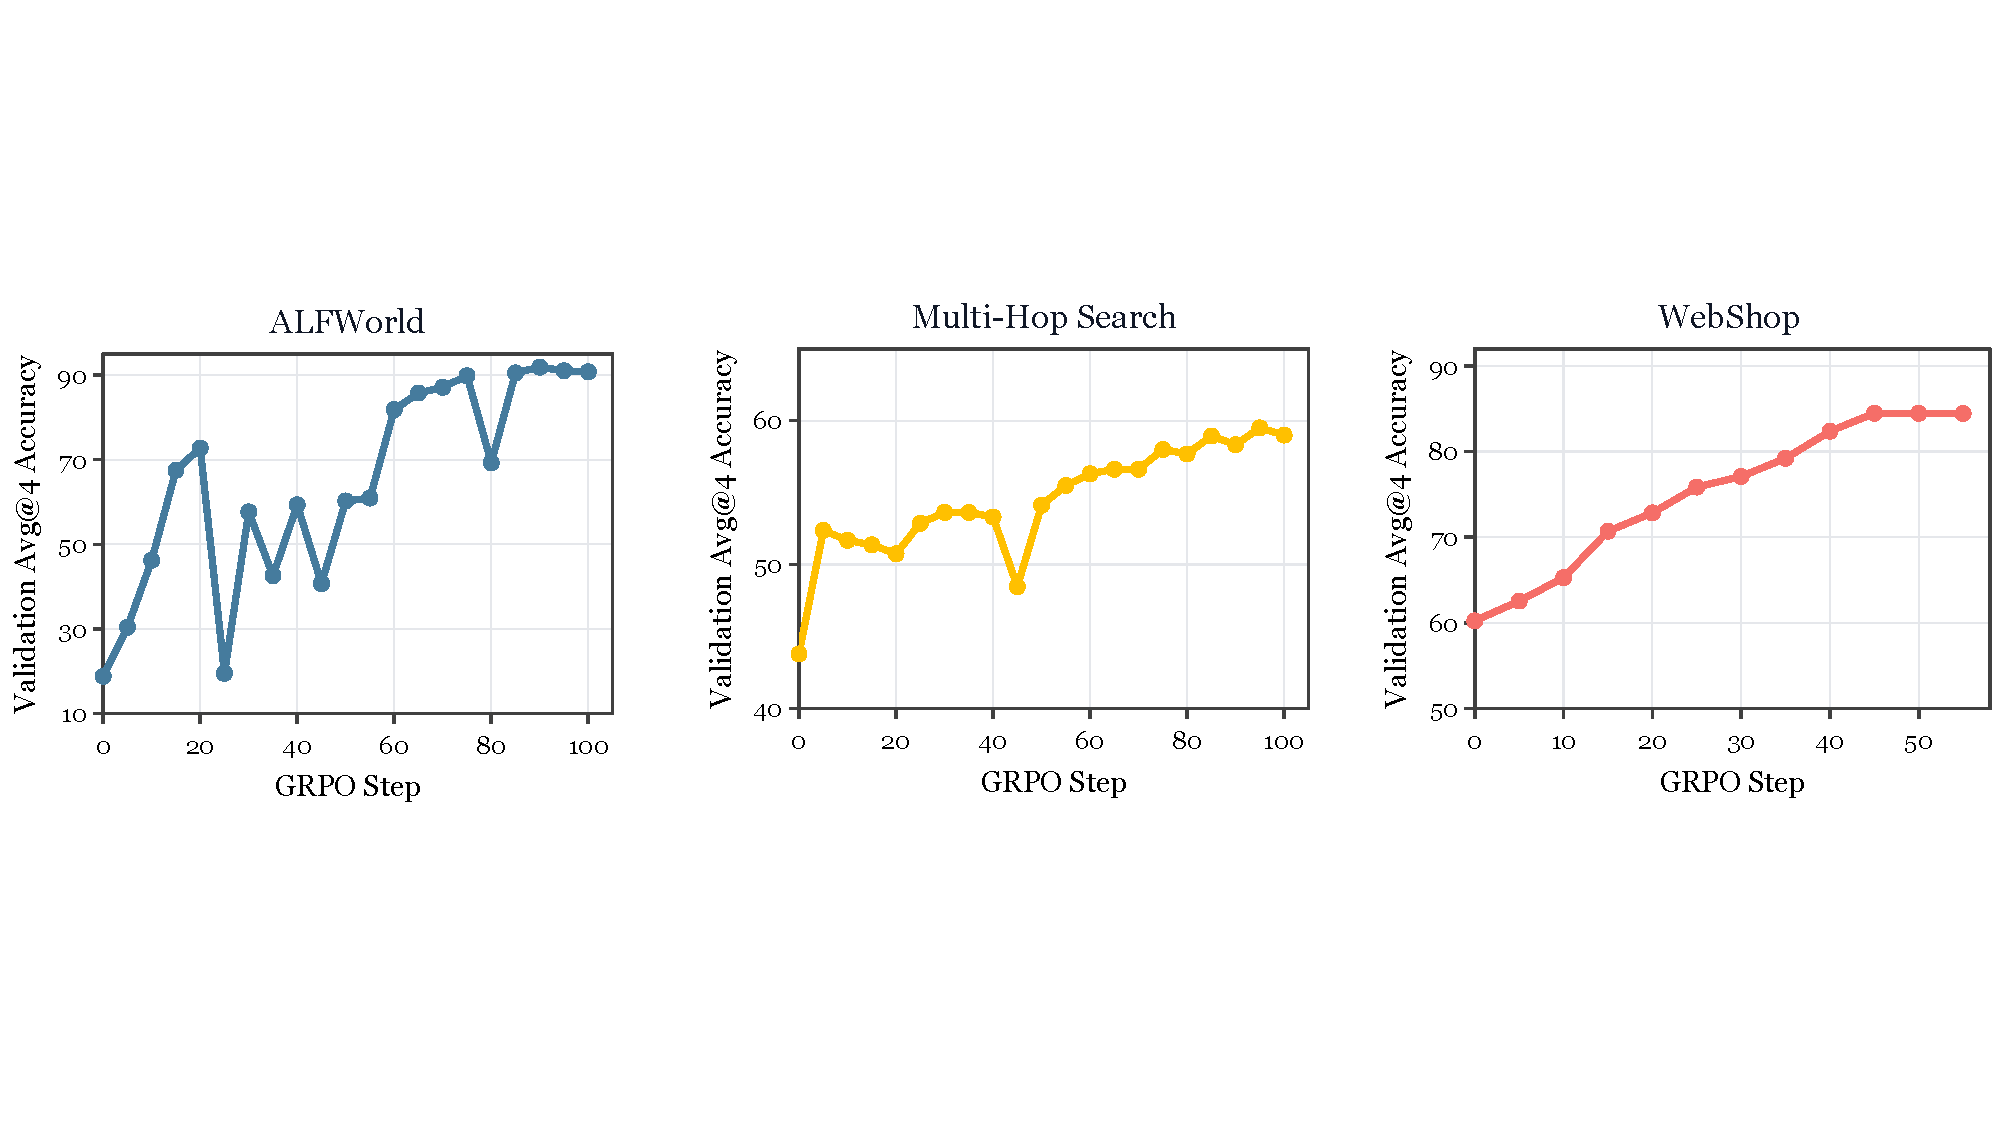
\includegraphics[width=\textwidth]{figures/grpo_training.pdf}
  \caption{GRPO validation curves for the task-specialized teacher models.}
  \label{fig:teacher-grpo-val}
\end{figure*}

\section{Proof Of The Contamination-Compression Bound}
\label{app:contamination-proof}

We provide the full proof of Proposition~\ref{prop:contamination-compression}.
Fix a context $c$ and write $\lambda=\lambda(c)$ for readability. The only
ingredient is the joint convexity of KL divergence. For any distributions
$P_1,Q_1,P_2,Q_2$ over the same vocabulary and any $\alpha\in[0,1]$,
\begin{equation}
\KL\!\left(\alpha P_1+(1-\alpha)P_2\,\|\,\alpha Q_1+(1-\alpha)Q_2\right)
\le
\alpha\KL(P_1\,\|\,Q_1)+(1-\alpha)\KL(P_2\,\|\,Q_2).
\label{eq:app-joint-convex-kl}
\end{equation}

\textbf{Joint convexity from log-sum.}
For each token $x$, set
$a_1=\alpha P_1(x)$, $a_2=(1-\alpha)P_2(x)$,
$b_1=\alpha Q_1(x)$, and $b_2=(1-\alpha)Q_2(x)$. The log-sum inequality gives
\begin{align}
&\big(a_1+a_2\big)
\log\frac{a_1+a_2}{b_1+b_2} \nonumber\\
&\qquad\le
a_1\log\frac{a_1}{b_1}
  + a_2\log\frac{a_2}{b_2} \nonumber\\
&\qquad=
\alpha P_1(x)\log\frac{P_1(x)}{Q_1(x)}
  +(1-\alpha)P_2(x)\log\frac{P_2(x)}{Q_2(x)} ,
\end{align}
where the factors $\alpha$ and $1-\alpha$ cancel inside the logarithms. Summing
over all tokens $x$ gives Equation~\ref{eq:app-joint-convex-kl}.

\textbf{Applying the inequality.}
Set $\alpha=\lambda$, $P_1=Q_1=p_F$, $P_2=p_S^{\mathrm{free}}$, and
$Q_2=p_T^{\mathrm{free}}$. Then
\begin{align}
&\KL\!\left(
\lambda p_F + (1-\lambda)p_S^{\mathrm{free}}
\,\|\,
\lambda p_F + (1-\lambda)p_T^{\mathrm{free}}
\right) \nonumber\\
&\qquad\le
\lambda \KL(p_F\,\|\,p_F)
  + (1-\lambda)\KL(p_S^{\mathrm{free}}\,\|\,p_T^{\mathrm{free}}).
\end{align}
Because $\KL(p_F\,\|\,p_F)=\sum_x p_F(x)\log 1=0$,
\begin{equation}
\KL\!\left(
\lambda p_F + (1-\lambda)p_S^{\mathrm{free}}
\,\|\,
\lambda p_F + (1-\lambda)p_T^{\mathrm{free}}
\right)
\le
(1-\lambda)\KL(p_S^{\mathrm{free}}\,\|\,p_T^{\mathrm{free}}),
\end{equation}
which proves Equation~\ref{eq:contamination-bound}.

\section{Existence of a Latent Rollout-Depth Optimum}
\label{app:rollout-depth-existence}

This appendix justifies the notation $H^\star$ used in
Section~\ref{sec:method}. The useful rollout horizon is not defined by a single
force. It is squeezed between two opposing requirements. If the horizon is too
short, the rollout fails to cover the decision turns on which successful
trajectories finish. If the horizon is too long, the remaining turns add
collection cost after the measurable teacher-correction signal has already
decayed. This gives a two-sided efficiency--coverage sandwich.

\textbf{Efficiency side.}
Fix a student checkpoint, a task distribution, and a finite maximum rollout cap
$H_{\max}$. For an idealized depth $H$, let
\begin{equation}
\rho(H)
  =
  \frac{\sum_{t\le H} v_t w_t}
       {\sum_{t\le H} c_t w_t+\epsilon},
\label{eq:app-efficiency-rate}
\end{equation}
where $v_t\ge0$ is the local teacher-correction value at turn $t$,
$w_t=n_t/n_0$ is the survivor probability, and $c_t>0$ is the per-turn
collection cost. Let $H_{\mathrm{eff}}^\star$ be the smallest maximizer of
$\rho(H)$ on $1\le H\le H_{\max}$. Equivalently, adding turn $H+1$ improves the
ratio only when its marginal rate is at least the current average:
\begin{equation}
\rho(H+1)\ge \rho(H)
\quad\Longleftrightarrow\quad
\frac{v_{H+1}}{c_{H+1}}\ge \rho(H),
\label{eq:app-marginal-rate}
\end{equation}
obtained by cross-multiplying
$(A+a)/(B+b)\ge A/B$ for positive $B,b$. Suppose there is a signal-exhaustion
frontier $\tau_c$ after which the marginal teacher-correction value is zero, or
more generally the marginal rate stays below the running average. Then every
turn beyond $\tau_c$ can only decrease the efficiency ratio, so
\begin{equation}
H_{\mathrm{eff}}^\star \le \tau_c-1 .
\label{eq:app-heff-upper}
\end{equation}

\textbf{Coverage side.}
Let $L_{\mathrm{succ}}$ be the completion length of a successful rollout, and
let
\begin{equation}
F_{\mathrm{succ}}(H)=\Pr(L_{\mathrm{succ}}\le H),\qquad
H_{\mathrm{cov}}=\widehat Q_p(L_{\mathrm{succ}})
  =\min\{H:F_{\mathrm{succ}}(H)\ge p\},
\label{eq:app-hcov}
\end{equation}
for a fixed $p\in(0,1]$. This is a coverage floor: stopping before
$H_{\mathrm{cov}}$ misses the completion decisions of more than a $(1-p)$
fraction of successful trajectories. Define the full-coverage completion depth
as
\begin{equation}
\tau_{\mathrm{done}}
  =
  \min\{H:F_{\mathrm{succ}}(H)=1\}.
\label{eq:app-tau-done}
\end{equation}
Equivalently, for a finite empirical support this is the largest observed
successful completion length, $\max\mathrm{supp}(L_{\mathrm{succ}})$. This
definition is deliberately the first point that has \emph{already} covered all
successful completions, not the last point before full coverage. Therefore
\begin{equation}
H_{\mathrm{cov}}\le \tau_{\mathrm{done}} .
\label{eq:app-hcov-upper}
\end{equation}

\textbf{Sandwich.}
The latent target should respect both sides:
\begin{equation}
H^\star
  =
  \max\!\left(H_{\mathrm{eff}}^\star,\ H_{\mathrm{cov}}\right).
\label{eq:app-hstar-sandwich-def}
\end{equation}
Therefore
\begin{equation}
H_{\mathrm{eff}}^\star
\le
H^\star
\le
\max\!\left(\tau_c-1,\tau_{\mathrm{done}}\right).
\label{eq:app-hstar-sandwich}
\end{equation}
The lower side prevents an overly shallow efficiency optimum from truncating
turns that successful trajectories need; the upper side prevents the horizon
from extending past both the signal-exhaustion frontier and the deepest
successful completion.


\section{Complete TurnOPD Hyperparameters}
\label{app:hyper}

Table~\ref{tab:hyper-full} lists the full configuration of the main TurnOPD method,
mapping each implementation key to the symbol used in the formal model
(Sections~\ref{sec:method:A}--\ref{sec:method:B}).
The \texttt{ema\_alpha} parameter is the EMA weight on the depth proxy
$H_{\mathrm{ctrl}}$, distinct from the loss-blend coefficient $\alpha$.

\begin{algorithm}[H]
  \small
  \caption{TurnOPD training algorithm.}
  \label{alg:tasc}
  \DontPrintSemicolon
  \KwIn{$\pi_\theta$, $\pi_T$, task distribution $\mathcal D$, rollout bounds
  $H_{\min},H_{\max}$, training horizon $K$, and controller hyperparameters
  $K_{\mathrm{warm}},r_{\mathrm{probe}},\alpha_{\mathrm{ema}},
  p,n_{\min}^{\mathrm{cov}},(s,e)$.}
  \KwOut{updated student policy $\pi_\theta$.}
  \BlankLine
  Initialize $\bar H_0 \leftarrow H_{\max}$ and $\Hcov \leftarrow 0$\;
  \For{$k=1$ \KwTo $K$}{
    $\hat H_k \leftarrow
    \mathrm{clip}(\mathrm{round}(\bar H_{k-1})+1,H_{\min},H_{\max})$\;
    $\mathrm{probe}_k \leftarrow (k\le K_{\mathrm{warm}})\ \lor\
    (k\bmod r_{\mathrm{probe}}=0)$\;
    \eIf{$\mathrm{probe}_k$}{
      $H_{\mathrm{roll}} \leftarrow H_{\max}$\;
    }{
      $H_{\mathrm{roll}} \leftarrow \hat H_k$\;
    }
    Collect on-policy trajectories $\mathcal B_k$ from $\pi_\theta$ on
    $\mathcal D$ up to $H_{\mathrm{roll}}$ turns\;
    Query $\pi_T$ on the supervised tokens in $\mathcal B_k$ and compute
    top-$K$ reverse-KL token losses $\ell_i$\;
    \If{$\mathrm{probe}_k$}{
      Compute per-turn raw-KL means $K_t$ and survivor counts $n_t$ from
      the uncensored probe batch\;
      $m_t \leftarrow [K_t]_+\,n_t/n_0$,\quad
      $q_t \leftarrow m_t/(\sum_j m_j+\epsilon)$\;
      $\Heff \leftarrow \mathrm{round}(\sum_t t\,q_t)$\;
      \If{$|\mathcal B_k^{\mathrm{succ}}|\ge n_{\min}^{\mathrm{cov}}$}{
        Estimate $F_{\mathrm{succ}}(H)$ from successful probe trajectories and set
        $\Hcov \leftarrow \min\{H:F_{\mathrm{succ}}(H)\ge p\}$\;
      }
      $H_{\mathrm{ctrl}} \leftarrow \max(\Heff,\Hcov)$\;
      $\bar H_k \leftarrow (1-\alpha_{\mathrm{ema}})\bar H_{k-1}
      +\alpha_{\mathrm{ema}}H_{\mathrm{ctrl}}$\;
    }
    \If{$\neg\,\mathrm{probe}_k$}{
      $\bar H_k \leftarrow \bar H_{k-1}$\;
    }
    $\rho_k \leftarrow k/K$,\quad
    $\alpha_k \leftarrow \mathrm{clip}((\rho_k-s)/(e-s),0,1)$\;
    Construct trajectory-normalized weights $w_{\mathrm{traj}}$ and
    turn-normalized weights $w_{\mathrm{turn}}$ on the observed tokens in
    $\mathcal B_k$\;
    $w_{\mathrm{blend}} \leftarrow
    (1-\alpha_k)w_{\mathrm{traj}}+\alpha_k w_{\mathrm{turn}}$\;
    $\mathcal L_k \leftarrow \sum_{i\in\mathcal B_k}
    w_{\mathrm{blend},i}\ell_i$\;
    Update $\theta$ by descending $\nabla_\theta \mathcal L_k$\;
  }
  \end{algorithm}


\begin{table*}[tbp]
\centering
\caption{Full TurnOPD configuration (ALFWorld-1.7B reference run). ``Symbol'' is the
variable in the formal model; ``Key'' is the implementation config name.}
\label{tab:hyper-full}
\scriptsize
\setlength{\tabcolsep}{3.5pt}
\resizebox{\textwidth}{!}{%
\begin{tabular}{@{}>{\centering\arraybackslash}m{2.8cm}>{\centering\arraybackslash}m{2.2cm}>{\centering\arraybackslash}m{5.3cm}>{\centering\arraybackslash}m{6.6cm}@{}}
\toprule
Group & Symbol & Key = value & Role \\
\midrule
\multirow{3}{*}{External signal}
 & $K_t$ & \texttt{kl\_per\_turn/*} & raw per-turn reverse-KL signal used in $m_t=[K_t]_+n_t/n_0$ \\
 & $n_t$ & \texttt{num\_traj/*} & all-trajectory survivor count used in the efficiency-side mass \\
 & $K_{\mathrm{top}}$       & \texttt{distill\_topk}=50 & teacher top-$K_{\mathrm{top}}$ support size for the reverse-KL loss \\
\midrule
\multirow{4}{*}{External depth}
 & $p$ & \texttt{coverage\_quantile}=0.80 & success-length quantile for $\Hcov=\hat Q_p(L_{\mathrm{succ}})$ \\
 & --- & \texttt{use\_success}=True & read $\Hcov$ from success subset (False $\to$ all-trajectory CDF) \\
 & --- & \texttt{min\_cov\_traj}=8 & min successful trajectories to refresh $\Hcov$ \\
 & $H_{\min}/H_{\max}$ & \texttt{min/max}=2/50 & clamp on applied depth $\hat H$ \\
\midrule
\multirow{3}{*}{External online}
 & $\alpha_{\mathrm{ema}}$ & \texttt{ema\_alpha}=0.30 & EMA weight on $H_{\mathrm{ctrl}}$ (not the blend $\alpha$) \\
 & --- & \texttt{probe\_interval}=8 & steps between full-depth probes \\
 & --- & \texttt{warmup\_steps}=3 & probe-only warmup before truncation \\
\midrule
\multirow{4}{*}{Internal blend}
 & $s,e$ & \texttt{blend start/end}=0/1 & linear progress window for $\alpha=\mathrm{clip}((\mathrm{prog}-s)/(e-s),0,1)$ \\
 & --- & \texttt{min\_floor}=8 & turn-level $n_{\min}=\max(\text{floor},\lceil\text{frac}\cdot n_{\mathrm{traj}}\rceil)$ \\
 & --- & \texttt{min\_frac}=0.15 & fraction term of $n_{\min}$ \\
 & --- & \texttt{turn\_norm\_blend}=True & enable linear trajectory$\to$turn blend \\
\midrule
\multirow{6}{*}{OPD / optimization}
 & --- & \texttt{kl\_coef}=0, \texttt{kl\_loss\_coef}=0 & no reward/penalty KL; loss is pure top-$K$ RKL \\
 & --- & \texttt{loss\_mode}=topk\_reverse\_kl & differentiable objective \\
 & --- & \texttt{seq-mean-token-mean} & base (trajectory-level) aggregation \\
 & --- & \texttt{clip\_ratio}=0.9/9 & importance-ratio clip (low/high) \\
 & --- & lr=$10^{-6}$, batch=64, steps=100 & AdamW \\
\midrule
\multirow{3}{*}{Rollout / eval}
 & --- & \texttt{max\_turns}=80 (ALFWorld) / 50 (Multi-Hop Search) & rollout turn cap before adaptive-depth truncation \\
 & --- & temperature=1.0, $n$=1 & training rollout sampling \\
 & --- & \texttt{val\_n}=4, val temp.=0.85 & validation: mean@4 \\
\bottomrule
\end{tabular}
}
\end{table*}

\FloatBarrier

\section{OPD Data Scale And Train/Test Construction}
\label{app:data}

Each task feeds the same on-policy distillation pipeline a parquet of prompts; the
agent then rolls out against the live environment, so a ``sample'' is a task
\textbf{instance} (a goal / question) rather than a fixed teacher trajectory---trajectories
are generated online during training. Table~\ref{tab:data} summarizes the reference
scale and split construction; the three tasks differ fundamentally in how their
train/test partitions are obtained, which we detail below.

\begin{table*}[tbp]
\centering
\caption{OPD dataset scale and split construction. ``Train/Eval'' counts are task
instances (online rollouts, not stored trajectories); the per-trajectory step cap is the
data-side \texttt{max\_iterations} before any adaptive-depth truncation.}
\label{tab:data}
\small
\setlength{\tabcolsep}{8pt}
\resizebox{\textwidth}{!}{%
\begin{tabular}{@{}>{\centering\arraybackslash}m{3.0cm}>{\centering\arraybackslash}m{2.2cm}>{\centering\arraybackslash}m{2.0cm}>{\centering\arraybackslash}m{6.8cm}@{}}
\toprule
Task & Train & Eval & Eval--train relation \\
\midrule
ALFWorld   & $\approx5000$ & $\approx300$ & held-out OOD split (\texttt{eval\_out\_of\_distribution}) \\
Multi-Hop Search  & $\approx30000$ & $\approx400$ & separate four-source QA test mixture \\
WebShop    & $\approx3000$ & $\approx200$ & disjoint goal-id ranges \\
\bottomrule
\end{tabular}
}
\end{table*}

\textbf{ALFWorld (procedurally generated, OOD evaluation).} Task instances are
synthesized by sampling one of the six task types uniformly
(Appendix~\ref{app:envs:alfworld}) and instantiating it with an object--receptacle pair
drawn from fixed vocabularies under a seeded RNG, so train and validation prompts are
reproducible and non-overlapping by seed. Crucially the two splits are routed to
\textbf{different} environment partitions: training instances use the \texttt{train}
games, whereas evaluation instances use the \texttt{eval\_out\_of\_distribution}
(valid-unseen) games, so reported accuracy measures generalization to unseen household
layouts rather than memorization. The reference configuration generates $\approx5000$
training and $\approx300$ evaluation instances with a per-trajectory step cap of $80$;
the underlying ALFWorld task pool has roughly $3.5\mathrm{k}$ unique games, which upper-bounds
the distinct training layouts.

\textbf{Multi-Hop Search (external QA mixture, separate test set).} Training uses an
externally prepared corpus of short-chain multi-hop / open-domain questions merged from
Search-R1-format sources, at $\approx30\mathrm{k}$ question--answer instances;
evaluation uses a separate held-out test set ($\approx400$ questions) drawn from
PopQA, Natural Questions (NQ), 2WikiMultiHopQA, and HotpotQA
(Appendix~\ref{app:envs:searchr1}), with the originating source preserved in the
\texttt{data\_source} field so that exact-match reward and per-source breakdowns route
correctly. Prompts are prepared with thinking enabled (a \texttt{<think>} reasoning
channel before each search), and the step cap is $50$ to accommodate several
search--read hops. Because the questions are real (not synthesized), train and test are
disjoint by construction at the dataset level.

\textbf{WebShop (goal-id partition, disjoint ranges).} A WebShop instance is selected
purely by a goal id (forwarded to the environment as the session/goal index); the
instruction text itself is part of the environment's initial observation and is not
duplicated into the prompt. Train and evaluation use \textbf{strictly disjoint} goal-id
ranges---evaluation takes ids $[0, N_{\mathrm{eval}})$ and training takes
$[N_{\mathrm{eval}}, N_{\mathrm{eval}}+N_{\mathrm{train}})$---so no goal appears in both
splits. The reference configuration uses $\approx3000$ training and $\approx200$
evaluation goals with a step cap of $30$ (WebShop episodes are short, typically 4--12
actions). Goal ids must stay within the goal count of the launched product corpus.

